% ILSVRC is exclusive, pascal is independent. this project attacks ilsvrc task 1 using pascal dataset.
% Dataset not augmented (e.g. rotation, blurring) since HEX paper didn't.
% hierarchy is form WordNet, exclusion is greedy
% realistic labelling assumption
% The authors of \cite{deng2014large} did not address this problem. In this work, accuracy is tested both in the extended concept space and the original one, by limiting the state space to those with an active bottom-level node.

\documentclass[11pt,a4paper]{article}
\usepackage{amsmath}
\usepackage{amssymb}
\usepackage{fullpage}
\usepackage{graphicx}
\usepackage[colorlinks=true, linkcolor=blue]{hyperref}

\newcommand{\argmin}{\operatornamewithlimits{arg\,min}}
\renewcommand{\arraystretch}{1.15} % line spacing in tabular

\begin{document}
\title{Improving Image Understanding with Concept Graph}
\author{Libo Yin\\The Australian National University}
\maketitle
\section{The Original HEX Model}

The original HEX model \cite{deng2014large} is an extension of the baseline flat multiclass classification model. There are two types of multiclass classification: exclusive, where the classifier predicts exactly one out of all possible states to be true; and independent, where each state is assigned true or false independently. HEX finds a balance between these two ends of the spectrum. It models the hierarchical and exclusive relationship between concepts, along with their hypernyms, with a semantic graph. Each node in this graph corresponds to a concept in the extended concept space being true or false. Due to the semantic constraints on the state of neighbouring nodes, the state space of HEX is much smaller than independent multiclass classification. HEX model classifies an image into a semantically consistent hierarchy. A simple HEX graph is shown in \hyperref[fig:naive]{figure~\ref{fig:naive}}.
\begin{figure}[h]
\centering
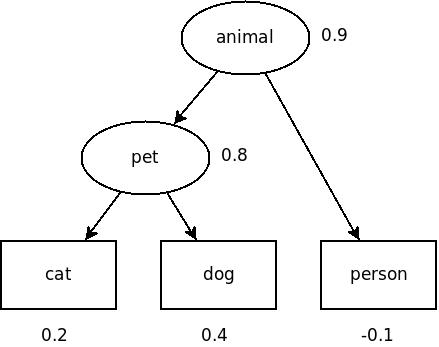
\includegraphics[scale=0.5]{naive.jpeg}
\caption{A simple HEX graph with three nodes in the original concept space (denoted by rectangles) and their hypernyms. Directed edges denote semantical hierarchy: $(a\rightarrow b)$ if $a$ is a hypernym of $b$; and undirected edges denote exclusion: $(a-b)$ if $a$ and $b$ cannot be true at the same time. Note that the hierarchical graph is in general a DAG rather than a tree.}
\label{fig:naive}
\end{figure}

Denoting the set of vertices by $V$, the set of hierarchical edges by $E_e$, and the set of exclusive edges by $E_h$, the joint assignment $y\in\{0,1\}^V$ can be defined as a CRF:
\[\tilde{p}(y|x)=\prod_{i\in V}\exp\{f_i(x;w)[y_i=1]\}\prod_{(v_i,v_j)\in E_h}[(y_i,y_j)\neq(0,1)]\prod_{(v_i,v_j)\in E_e}[(y_i,y_j)\neq(1,1)]\]

where $f_i(x;w)$ is a convolutional neural network. For notational convenience, we define:
\[I[y\text{ legal}]=\prod_{(v_i,v_j)\in E_h}[(y_i,y_j)\neq(0,1)]\prod_{(v_i,v_j)\in E_e}[(y_i,y_j)\neq(1,1)]\]

There are a few important observations about this potential function, listed below from most obvious to most surprising:
\begin{enumerate}
\item There are no learnable variables in this CRF.
\item Mathematically, CRF requires $\forall y:\tilde{p}(y|x)>0$. However, computationally, assigning zero to $\tilde{p}(y|x)$ can be interpreted as assigning an infinitesimal value. Therefore, the above definition is computationally equivalent to a legitimate CRF.
\item A valid state does not have to have an active node in the original concept space. For example, valid states of the HEX graph shown in \hyperref[fig:naive]{figure~\ref{fig:naive}} are:
\begin{enumerate}
\item $\varnothing$
\item \{animal\}
\item \{animal, pet\}
\item \{animal, person\}
\item \{animal, pet, cat\}
\item \{animal, pet, dog\}
\end{enumerate}

This allows an image to be classified to abstract concepts (even $\varnothing$) when the classifier is not confident to classify to anything in the original concept space. This is by no doubt a desirable feature for deployment. However, since all testing images are labelled in the original concept space, classifying to the extended concept space makes performance evaluation troublesome.
\item In \hyperref[fig:naive]{figure~\ref{fig:naive}}, the competition between state \{animal, pet, cat\} and \{animal, pet, dog\} depends entirely on the confidence of bottom-level node\footnote{Since hierarchical graph is not necessary a tree, ``leaf nodes'' is not an appropriate term here.} dog and cat. However, to discriminate between \{animal, pet, dog\} and \{animal, person\} requires examining the confidence along the path. From this process it can be seen that classifier confidence being passed down the hierarchy from abstract concept to concrete ones. On the other side of the same coin, during the CNN training stage, branching nodes receive more training data, and therefore gain more confidence. This can be seen as confidence being passed up in the hierarchy.
\item Consider the situation in \hyperref[fig:depth]{figure~\ref{fig:depth}}:
\begin{figure}[h]
\centering
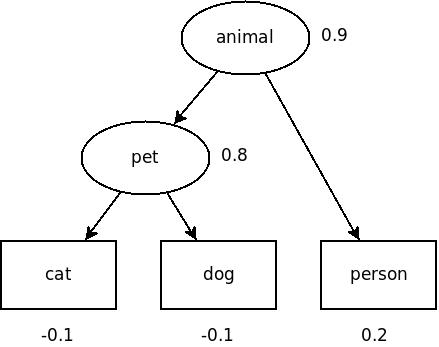
\includegraphics[scale=0.5]{depth.jpeg}
\caption{Numbers are confidence.}
\label{fig:depth}
\end{figure}

The classifier will classify to \{animal, pet, dog\}, not because the confidence is higher, but because there are more nodes along the path.

\item the greedy nature of potential function guarantees a bottom-level node to be activated
\end{enumerate}

In general, the HEX model can be seen as a noise filter that suppresses inconsistent results, and encourage consistent ones. The inference is by loopy belief propagation. This model turns out to be particularly beneficial for realistically labelled dataset, where mechanical turk tend to label an image to a more general term (e.g.\ ``Labrador'' as ``dog''). The basic steps are repeated as follows:

Let the set of ImageNet labels be $\mathcal{L}$. With WordNet, collect the hypernyms, transitively, of each concept in $\mathcal{L}$. 

It creates a semantic graphical model with classes as leaf nodes and hypernymes as branching nodes. The potential function is defined as follows:
\[\tilde{p}(y|x)=\prod_{i\in V}\exp\{f_i(x;w)[y_i=1]\}\prod_{(v_i,v_j)\in E_h}[(y_i,y_j)\neq(0,1)]\prod_{(v_i,v_j)\in E_e}[(y_i,y_j)\neq(1,1)]\]

For notational convenience, we define:
\[I[y\text{ legal}]=\prod_{(v_i,v_j)\in E_h}[(y_i,y_j)\neq(0,1)]\prod_{(v_i,v_j)\in E_e}[(y_i,y_j)\neq(1,1)]\]

To solve the hierarchy depth problem, we define:
\[\tilde{p}(y|x)=[y\text{ legal}]\prod_i\exp\{f_i(x;w)[y_i=1]+(1-f_i(x;w))[y_i=0]\}\]

We can see from the potential function that both hierarchical and exclusion edges help to reduce the label space, yet information only flows on hierarchy edges. The inference in original paper is LBP, where clique states are limited by the state space. On PASCAL, the inference is by brute force, due to the tiny state space.

\section{Improvements}

There are two issues in Deng's paper. First, the potential function does not handle different depth problem, and is greedy in labelling to bottom-layer nodes. As shall be discussed later, this has similar effects to reducing the state space, and is not a desired thing. Second, the inference system has no learnable part.

To fix the first problem, we redefine the potential function to consider not only the active nodes, but also the inactive ones. However, this fix contradicts with the realistic labelling assumption. Deng's paper assumes that a high proportion of images are actually labelled to their immediate parents, e.g. Husky are labelled as dog. As a result, the bottom layer classifiers (I did not use word "leaf layer" because the hierarchy graph is a DAG in general, and HEX is a loopy CRF. In the case of PASCAL, it happens to be a forest.) have very low confidence, due to the lack of training data. As a result, stopping at the next-to-bottom layer is almost always more preferable.

Of course, this problem can be fixed by limiting the state space to those with one active bottom-layer node. With this fix, the advantage of revised potential function is clear. However, this fix removed one of the core advantages of the HEX model: the possibility to label to an intermediate node, when the classifier is not confident enough to classify to a bottom-layer node.

On this issue, there is one more point to make. All of the ImageNet or PASCAL labels are on the bottom-layer. If the classifier is allowed to label an image to an intermediate layer, then the label space is enlarged. While this can be problematic during the validation and testing stage, it is without doubt a desirable feature during the deploy stage.

To sum up here, with little confidence on the bottom layer classifiers, the problem is to attempt to classify to the bottom layers. However, in case the classifier really cannot make a decision, it should be allowed to stop at an intermediate layer. In addition, the classifier should consider both active and inactive nodes.

Use all images to train the CNN, and images labelled to leaf nodes to train the CRF. Computation of partition function is by brute force, thanks to the tiny state space of PASCAL. Binary weights in the learned model should not suffer from the depth problem, as weights are able to adjust themselves.

\section{Dataset}

Not augmented by rotation or flip since the original paper didn't

\section{HEX with learning}

\[\theta=\argmin_\theta\left\{-\frac{C}{N}\log\prod_{(x,y)\in D}p_\theta(y|x)+\frac{1}{2}\|\theta\|^2\right\}\]

\begin{align*}
p_\theta(y|x)=\frac{1}{Z(x)}&\exp\left\{\frac{1}{|V|}\sum_{i\in V}w_i\big(x_i\cdot I[y_i=1]+(1-x_i)\cdot I[y_i=0]\big)\right\}\\
\cdot&\exp\left\{\frac{1}{|E|}\sum_{(i,j)\in E}t_{ij}\cdot x_ix_j\cdot I[y_i=y_j=1]\right\}\cdot I[y\text{ legal}]
\end{align*}

\begin{align*}
\log p_\theta(y|x)&=\frac{1}{|V|}\sum_{i\in V}w_i(x_i\cdot I[y_i=1]+(1-x_i)\cdot I[y_i=0])\\
&\quad+\frac{1}{|E|}\sum_{(i,j)\in E}t_{ij}\cdot x_ix_j\cdot I[y_i=y_j=1]-\log\sum_{\hat{y}}\tilde{p}_\theta(\hat{y}|x)
\end{align*}

\begin{align*}
\nabla_\theta\log\prod_{(x,y)\in D}p_\theta(y|x)&=\begin{bmatrix}
\nabla_w\log\prod_{(x,y)\in D}p_\theta(y|x)\\ 
\nabla_t\log\prod_{(x,y)\in D}p_\theta(y|x)
\end{bmatrix}\\
&=\begin{bmatrix}
\sum_{(x,y)\in D}\nabla_w\log p_\theta(y|x)\\ 
\sum_{(x,y)\in D}\nabla_t\log p_\theta(y|x)
\end{bmatrix}
\end{align*}

\begin{align*}
\nabla_w\log p_\theta(y|x)&=\underbrace{\frac{1}{|V|}\Big[x_i\cdot I[y_i=1]+(1-x_i)\cdot I[y_i=0]\Big]_{i\in V}}_{\phi_u(x,y)}-\nabla_w\log\sum_{\hat{y}}\tilde{p}_\theta(\hat{y}|x)\\
&=\phi_u(x,y)-\sum_{\hat{y}}p_\theta(\hat{y}|x)\cdot\phi_u(x,\hat{y})
\end{align*}

\begin{align*}
\nabla_w\log\sum_{\hat{y}}\tilde{p}_\theta(\hat{y}|x)&=\frac{1}{\sum_{\hat{y}}\tilde{p}_\theta(\hat{y}|x)}\nabla_w\sum_{\hat{y}}\tilde{p}_\theta(\hat{y}|x)\\
&=\frac{1}{Z(x)}\sum_{\hat{y}}\nabla_w\exp\left\{\frac{1}{|V|}\sum_{i\in V}w_i\big(x_i\cdot I[y_i=1]+(1-x_i)\cdot I[y_i=0]\big)\right\}\\
&\quad\cdot\exp\left\{\frac{1}{|E|}\sum_{(i,j)\in E}t_{ij}\cdot x_ix_j\cdot I[y_i=y_j=1]\right\}\\
&=\frac{1}{Z(x)}\sum_{\hat{y}}\tilde{p}_\theta(\hat{y}|x)\cdot\frac{1}{|V|}\Big[x_i\cdot I[\hat{y}_i=1]+(1-x_i)\cdot I[\hat{y}_i=0]\Big]_{i\in V}\\
&=\sum_{\hat{y}}p_\theta(\hat{y}|x)\cdot\phi_u(x,\hat{y})
\end{align*}

\begin{align*}
\nabla_t\log p_\theta(y|x)&=\underbrace{\frac{1}{|E|}\Big[t_{ij}\cdot x_ix_j\cdot I[y_i=y_j=1]\Big]_{(i,j)\in E}}_{\phi_t(x,y)}-\nabla_t\log\sum_{\hat{y}}\tilde{p}_\theta(\hat{y}|x)\\
&=\phi_t(x,y)-\sum_{\hat{y}}p_\theta(\hat{y}|x)\cdot\phi_t(x,\hat{y})
\end{align*}

\begin{align*}
\nabla_t\log\sum_{\hat{y}}\tilde{p}_\theta(\hat{y}|x)&=\frac{1}{\sum_{\hat{y}}\tilde{p}_\theta(\hat{y}|x)}\nabla_t\sum_{\hat{y}}\tilde{p}_\theta(\hat{y}|x)\\
&=\frac{1}{Z(x)}\sum_{\hat{y}}\nabla_t\exp\left\{\frac{1}{|V|}\sum_{i\in V}w_i\big(x_i\cdot I[y_i=1]+(1-x_i)\cdot I[y_i=0]\big)\right\}\\
&\quad\cdot\exp\left\{\frac{1}{|E|}\sum_{(i,j)\in E}t_{ij}\cdot x_ix_j\cdot I[y_i=y_j=1]\right\}\\
&=\frac{1}{Z(x)}\sum_{\hat{y}}\tilde{p}_\theta(\hat{y}|x)\cdot\frac{1}{|E|}\Big[t_{ij}\cdot x_ix_j\cdot I[\hat{y}_i=\hat{y}_j=1]\Big]_{(i,j)\in E}\\
&=\sum_{\hat{y}}p_\theta(\hat{y}|x)\cdot\phi_t(x,\hat{y})
\end{align*}

\appendix
\section{Attributed HEX}

In earlier stages of this project, one of the proposed directions is the joint analysis of concept and attributes. That is, for example, to classify an image of yellow Labrador into ``animal, pet, dog, yellow, hasFur'', etc. An example HEX graph is shown as follows:

While the training data is provided by UIUC's aPascal \& aYahoo dataset. [TODO: cite dataset, discuss dataset properties] The possibility of using CNN as feature extractor has been confirmed in [TODO: cite].

We only connected attributes to bottom-level concepts. In other words, the aHEX graph can be seen as a semantic part and an attribute part. Such design is for the sake of reducing loops in the aHEX graph. While junction-tree algorithm could potentially handle such a loopy graph during inference stage, the loops makes the graph very tricky to learn as a CRF. Similar design has been applied to pixel labelling problem such as [TODO: find references].

However, it was not the loops that caused such idea to be dropped. Under the same non-learning model, potential function is submodular, therefore such extension s trivial. Under the learnable CRF model, the aHEX graph can be learned part-wise: the semantic subgraph can be learned in the same way as discussed in [TODO: cross-ref learnable CRF], whereas for the attributes part, all bottom-level concepts can be grouped into a super-concept with 20 states (corresponding to 20 PASCAL labels), then the attribute graph becomes a tree, which is learnable[TODO: find references]. With such model, the inference is the same as an non-learning system, as the potential function for the attributed part still has a submodular structure.

\section{Probabilistic HEX}

Afte the ECCV 14 paper, the original authors extended HEX to pHEX by relaxing 0/1 hard constraints to $u\in(0,1)$, and turning the HEX graph into an Ising model. pHEX managed to beat HEX by [TODO]. However, the crucial $u$ is chosen by cross-validation, and it still applies to all constraints in the graph. In addition, pHEX require a long time to train, although still much shorter than training the underlying CNN. Also, it uses the same potential function as original HEX. Compared to pHEX, this work focuses on using a more flexible potential function. In term of running time, these two works are not directly comparable since this work is not scalable.

\clearpage
\bibliographystyle{plain}
\bibliography{ref}
\end{document}